\documentclass[11pt]{article}

\usepackage[margin=0.78in]{geometry}
\usepackage[T1]{fontenc}
\usepackage[utf8]{inputenc}
\usepackage{amsmath,amssymb,mathtools}
\usepackage{microtype}
\usepackage{xcolor}
\usepackage{enumitem}
\usepackage{booktabs}
\usepackage{graphicx}
\usepackage{float}
\usepackage{caption}
\usepackage{subcaption}
\usepackage{hyperref}
\usepackage{tikz}
\usetikzlibrary{arrows.meta,positioning,calc,fit}

% Compile from grpo_experiments/
\graphicspath{{./writeup_package/figures/}{./figures/}}

\hypersetup{
    colorlinks=true,
    linkcolor=blue!45!black,
    urlcolor=blue!45!black
}

\setlength{\parindent}{0pt}
\setlength{\parskip}{0.38em}
\setlist[itemize]{leftmargin=1.5em,itemsep=0.15em,topsep=0.25em}
\setlist[enumerate]{leftmargin=1.7em,itemsep=0.15em,topsep=0.25em}

\newcommand{\PF}{P_F}
\newcommand{\PB}{P_B}
\newcommand{\qphi}{q_\phi}
\newcommand{\Tset}{\mathcal{T}}
\newcommand{\R}{R}

\definecolor{accent}{RGB}{46,91,132}
\definecolor{softaccent}{RGB}{235,243,249}

\tikzset{
    flowbox/.style={
        draw,
        rounded corners,
        align=center,
        fill=white,
        inner sep=5pt,
        font=\small
    },
    keybox/.style={
        flowbox,
        draw=accent,
        thick,
        fill=softaccent
    },
    arrow/.style={
        -{Latex[length=2mm]},
        thick,
        draw=accent
    },
    lightarrow/.style={
        -{Latex[length=1.8mm]},
        draw=black!60
    },
    backarrow/.style={
        -{Latex[length=1.8mm]},
        dashed,
        draw=black!60
    }
}

\title{\textbf{Learning a Reverse Policy for Trajectory-Level IPS}\\
\large Algorithm, Methodology, and Results}
\author{}
\date{}

\begin{document}
\maketitle

\section*{Overview}

This note explains the role of the learned reverse policy \(\qphi(\tau\mid x)\) in trajectory-level inverse probability scaling, and then reports the algorithm, methodology, and results. The main difficulty is that the forward policy gives probabilities for complete trajectories, while the learning objective is defined over terminal outputs. Since many trajectories may lead to the same terminal, directly using a trajectory probability overcounts terminals that can be reached through more paths.

The reverse policy solves this problem by defining a normalized distribution over all trajectories that could have produced a terminal \(x\). Its normalization gives the correct terminal-level weighted target. We then learn the reverse policy from on-policy forward trajectories so that it better matches the paths used by the forward policy and reduces the variance of the importance weights.

We first validate the method on a controlled toy DAG, where the ideal target is known exactly, and then apply it as a first domain application to phylogenetic tree construction (PhyloGFN).

%======================================================================
\section{Setup}
\label{sec:setup}
%======================================================================

The environment is represented as a directed acyclic graph (DAG). Each node is a state, each directed edge is an action, and every episode starts from a fixed root state. The forward policy generates a trajectory
\begin{equation}
    \tau=(s_0,a_1,s_1,\ldots,a_T,s_T),
\end{equation}
ending at the terminal output
\begin{equation}
    x=s_T.
\end{equation}

Our goal is to make terminal outputs appear in proportion to their rewards:
\begin{equation}
    p^*(x)=\frac{\R(x)}{Z},
    \qquad
    Z=\sum_x \R(x).
    \label{eq:terminal-target}
\end{equation}

The forward policy induces a path probability
\begin{equation}
    \PF(\tau)
    =
    \prod_{t=1}^{T}\PF(a_t\mid s_{t-1}),
    \label{eq:forward-path-probability}
\end{equation}
and a terminal marginal
\begin{equation}
    \PF(x)
    =
    \sum_{\tau\in\Tset(x)}\PF(\tau),
    \label{eq:terminal-probability}
\end{equation}
where \(\Tset(x)\) is the set of all trajectories ending at \(x\).

If \(\PF(x)\) were available, the ideal inverse-probability weight would be
\begin{equation}
    w(x)=\frac{\R(x)}{\PF(x)}.
\end{equation}
Computing \(\PF(x)\) requires summing over all trajectories that end at \(x\). This is possible by enumeration or dynamic programming in the small toy DAG, but is impractical in large or implicit state spaces such as phylogeny.

%======================================================================
\section{Problem: trajectory probability is not terminal probability}
\label{sec:multiplicity}
%======================================================================

\begin{figure}[t]
\centering
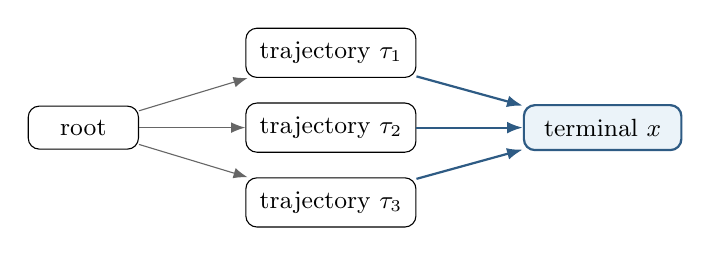
\begin{tikzpicture}[node distance=0.75cm and 1.35cm]
    \node[flowbox, minimum width=1.4cm] (root) {root};
    \node[flowbox, right=of root, yshift=0.95cm] (t1) {trajectory $\tau_1$};
    \node[flowbox, right=of root] (t2) {trajectory $\tau_2$};
    \node[flowbox, right=of root, yshift=-0.95cm] (t3) {trajectory $\tau_3$};
    \node[keybox, right=1.35cm of t2, minimum width=2.0cm] (x) {terminal $x$};

    \draw[lightarrow] (root) -- (t1);
    \draw[lightarrow] (root) -- (t2);
    \draw[lightarrow] (root) -- (t3);
    \draw[arrow] (t1) -- (x);
    \draw[arrow] (t2) -- (x);
    \draw[arrow] (t3) -- (x);
\end{tikzpicture}
\caption{The mapping from trajectories to terminal outputs is generally many-to-one.}
\label{fig:trajectory-terminal}
\end{figure}

For a sampled rollout, \(\PF(\tau)\) is known exactly. A tempting alternative is therefore
\begin{equation}
    w_{\mathrm{naive}}(\tau)
    =
    \frac{\R(x)}{\PF(\tau)}.
\end{equation}
This gives the wrong weighted target. For every trajectory ending at \(x\),
\begin{equation}
    \PF(\tau)
    \frac{\R(x)}{\PF(\tau)}
    =
    \R(x).
\end{equation}
Therefore, the reward is counted once for every trajectory leading to \(x\). If
\begin{equation}
    m(x)=|\Tset(x)|
\end{equation}
is the number of such trajectories, the total weighted contribution becomes \(m(x)\R(x)\) rather than \(\R(x)\). Terminals with more possible paths receive too much target mass.

\begin{center}
\fbox{%
\begin{minipage}{0.88\textwidth}
\centering
Using \(\R(x)/\PF(\tau)\) counts the reward once per trajectory, while the objective requires it to be counted once per terminal output.
\end{minipage}}
\end{center}

This multiplicity problem appears in both domains studied here:
\begin{itemize}
    \item \textbf{Toy DAG:} with budget \(B=3\) and max step \(K=3\), the four terminals have multiplicities \((4,5,5,4)\).
    \item \textbf{Phylogeny:} for 5 taxa, \(m(x)\) ranges from 8 to 48 depending on topology; at 27 taxa, \(m(x)\) is enormous and cannot be computed.
\end{itemize}

%======================================================================
\section{Solution: a normalized reverse distribution}
\label{sec:reverse}
%======================================================================

We introduce a reverse distribution
\begin{equation}
    \qphi(\tau\mid x),
\end{equation}
which assigns probabilities to the possible trajectories that could have produced terminal \(x\). For each terminal, it satisfies
\begin{equation}
    \sum_{\tau\in\Tset(x)}\qphi(\tau\mid x)=1.
    \label{eq:q-normalized}
\end{equation}

The corrected importance weight is
\begin{equation}
    w(\tau)
    =
    \frac{\R(x)\,\qphi(\tau\mid x)}{\PF(\tau)}.
    \label{eq:corrected-weight}
\end{equation}

The total weighted contribution of all trajectories ending at \(x\) is
\begin{align}
    \sum_{\tau\in\Tset(x)}\PF(\tau)w(\tau)
    &={}
    \sum_{\tau\in\Tset(x)}
    \PF(\tau)
    \frac{\R(x)\qphi(\tau\mid x)}{\PF(\tau)}
    \\
    &={}
    \R(x)
    \sum_{\tau\in\Tset(x)}\qphi(\tau\mid x)
    \\
    &={}
    \R(x).
\end{align}

Thus, the total target mass assigned to a terminal depends on its reward, not on the number of trajectories that lead to it.

Equivalently, define the trajectory-level target distribution
\begin{equation}
    p_\phi^*(\tau)
    =
    \frac{
        \R(x(\tau))\qphi(\tau\mid x(\tau))
    }{Z}.
\end{equation}
Its terminal marginal is
\begin{equation}
    \sum_{\tau\in\Tset(x)}p_\phi^*(\tau)
    =
    \frac{\R(x)}{Z}.
\end{equation}

The choice of \(\qphi\) changes how mass is distributed among trajectories leading to the same terminal, but it does not change the total mass assigned to that terminal.

\begin{center}
\fbox{%
\begin{minipage}{0.88\textwidth}
\centering
\textbf{Normalization makes \(\qphi\) correct at the terminal level. Learning \(\qphi\) reduces the variance of the weights.}
\end{minipage}}
\end{center}

\paragraph{Why learn \(\qphi\) rather than fix it uniform?}
A fixed uniform reverse policy is valid, but typically far from the forward conditional \(\PF(\tau\mid x)\). When \(\qphi\neq \PF(\cdot\mid x)\), weights vary across paths to the same terminal, inflating variance and reducing effective sample size (ESS). When \(\qphi=\PF(\tau\mid x)\),
\begin{equation}
    w(\tau)
    =
    \frac{\R(x)\,\PF(\tau\mid x)}{\PF(x)\,\PF(\tau\mid x)}
    =
    \frac{\R(x)}{\PF(x)},
\end{equation}
which is constant across all paths to \(x\) --- zero within-terminal variance.

\paragraph{Correctness vs.\ variance.}
A poorly fit \(\qphi\) increases weight variance but \textbf{cannot bias the terminal marginal}, because normalization over paths to \(x\) holds for any \(\phi\). Learning \(\qphi\) is therefore a variance-reduction strategy on top of a valid estimator.

%======================================================================
\section{How \(\qphi\) is learned}
\label{sec:learning}
%======================================================================

We learn \(\qphi\) by treating sampled forward trajectories as training data for a reverse classification problem.

\subsection{What is collected from on-policy trajectories}

At each training iteration, the current forward policy samples a batch of trajectories
\begin{equation}
    \tau_i
    =
    (s_{i,0},a_{i,1},s_{i,1},\ldots,a_{i,T_i},s_{i,T_i}),
    \qquad
    x_i=s_{i,T_i}.
\end{equation}

For every trajectory, we record:
\begin{itemize}
    \item the visited states \(s_{i,0},\ldots,s_{i,T_i}\);
    \item the actions \(a_{i,1},\ldots,a_{i,T_i}\);
    \item the terminal output \(x_i\);
    \item the terminal reward \(\R(x_i)\);
    \item the forward action log-probabilities, whose sum gives
    \begin{equation}
        \log \PF(\tau_i)
        =
        \sum_{t=1}^{T_i}
        \log \PF(a_{i,t}\mid s_{i,t-1}).
    \end{equation}
\end{itemize}

The reward and forward trajectory probability are used to construct the IPS weight. They are not used in the reverse-policy loss.

\subsection{Converting a trajectory into reverse examples}

Every edge of a sampled trajectory gives one labelled reverse example:
\begin{equation}
    \underbrace{(s_{i,t},x_i)}_{\text{input}}
    \quad\longrightarrow\quad
    \underbrace{a_{i,t}}_{\text{observed incoming edge}}.
    \label{eq:edge-example}
\end{equation}

The child state \(s_{i,t}\) tells the reverse model where it currently is, and the terminal \(x_i\) tells it which final output the full trajectory produced. A mask identifies which parent edges are valid at \(s_{i,t}\).

The reverse network outputs a masked categorical distribution over possible incoming actions:
\begin{equation}
    \qphi(a\mid s_{i,t},x_i).
\end{equation}
Multiplying these edge probabilities gives the reverse probability of the complete trajectory:
\begin{equation}
    \qphi(\tau_i\mid x_i)
    =
    \prod_{t=1}^{T_i}
    \qphi(a_{i,t}\mid s_{i,t},x_i).
    \label{eq:q-path-product}
\end{equation}
In practice, this is calculated in log space:
\begin{equation}
    \log \qphi(\tau_i\mid x_i)
    =
    \sum_{t=1}^{T_i}
    \log \qphi(a_{i,t}\mid s_{i,t},x_i).
    \label{eq:q-path-log}
\end{equation}

\begin{figure}[p]
\centering
\resizebox{0.98\textwidth}{!}{%
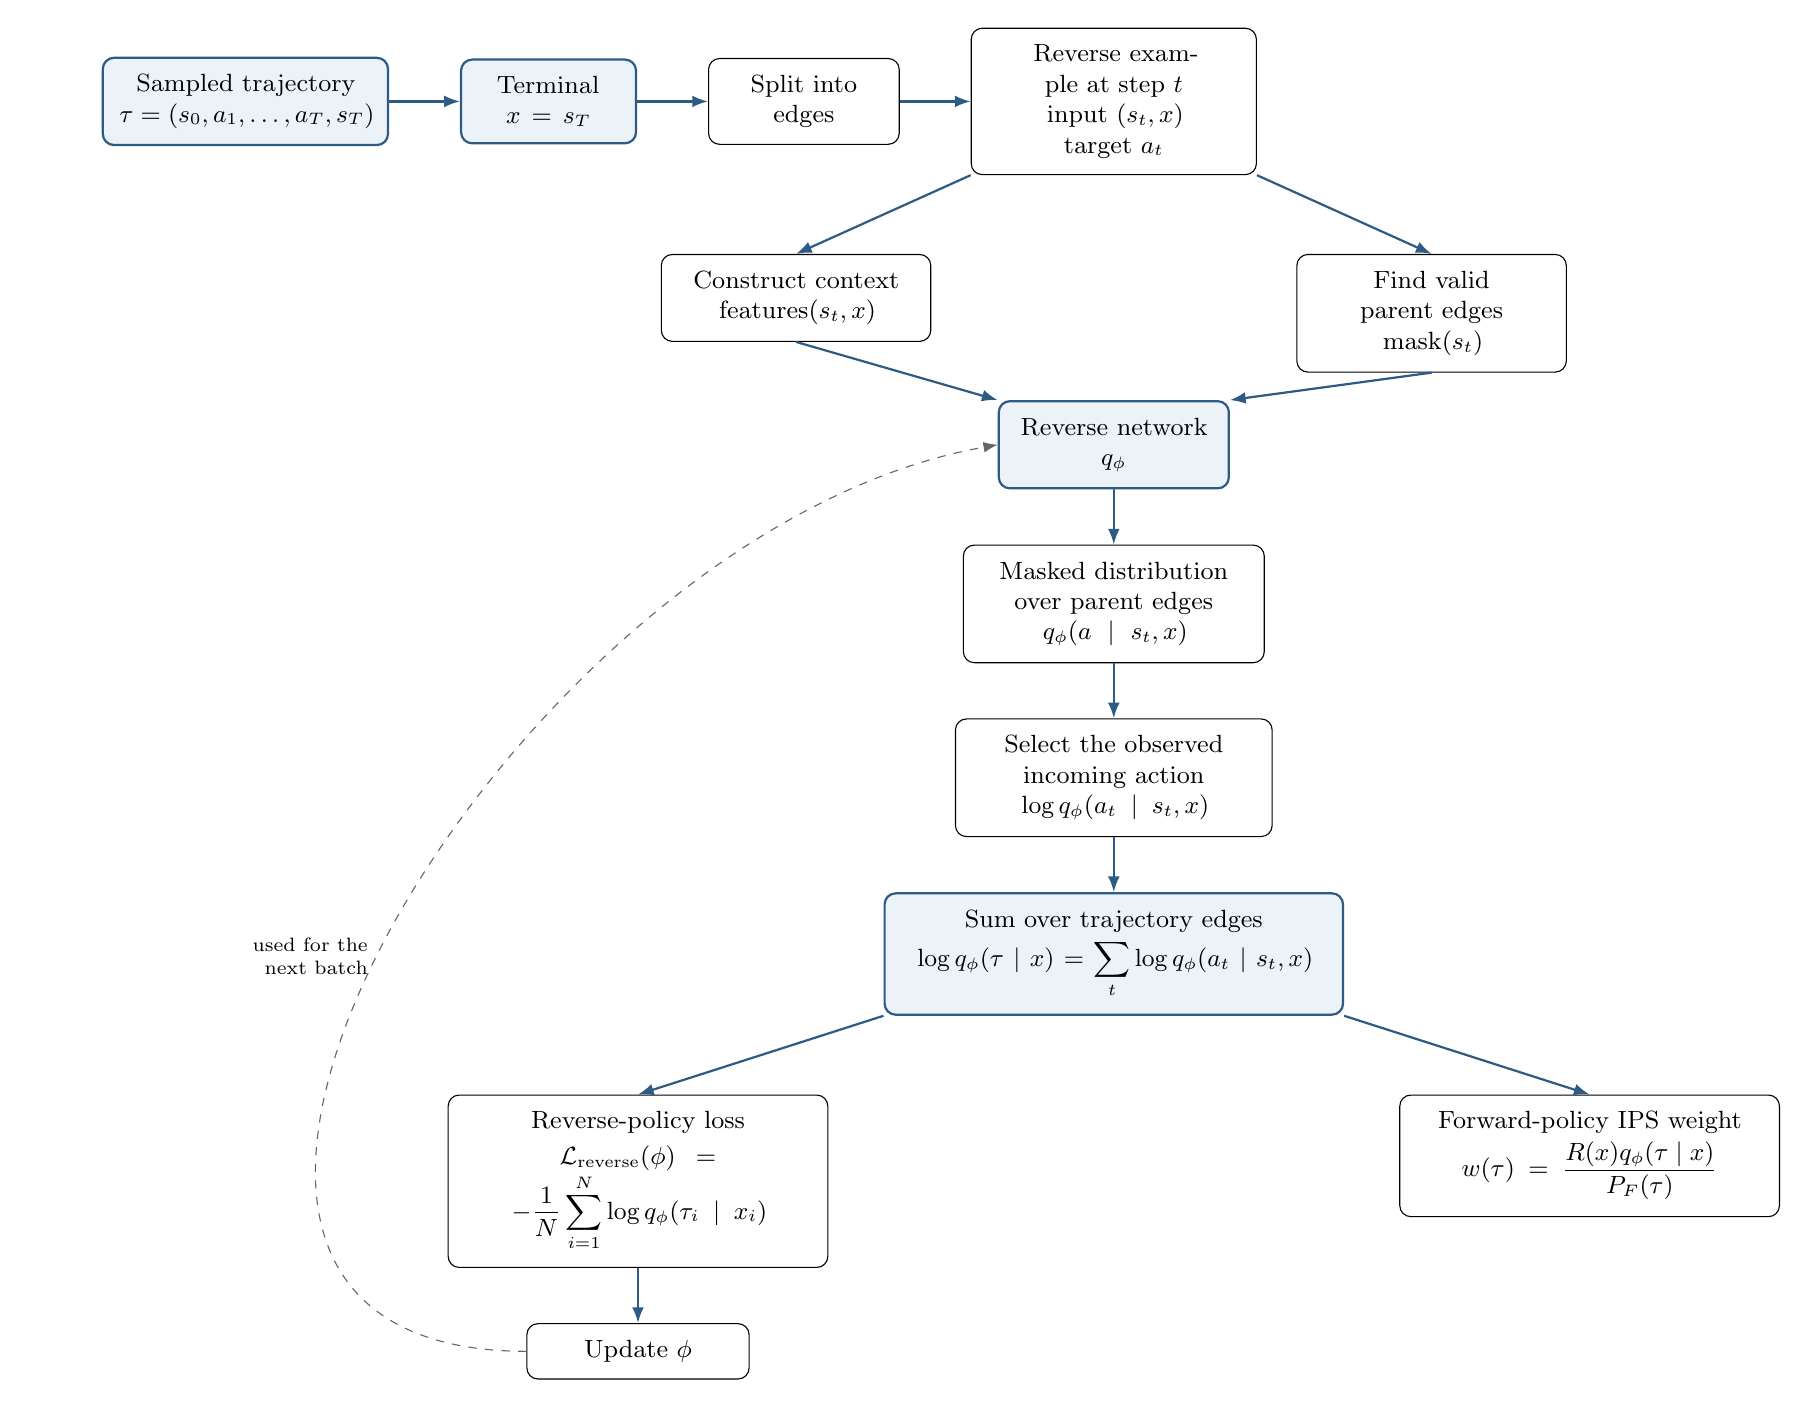
\begin{tikzpicture}[
    node distance=7mm and 9mm,
    every node/.append style={font=\small},
    flowbox/.append style={inner sep=6pt},
    keybox/.append style={inner sep=6pt}
]
    \node[keybox, text width=3.2cm] (traj)
        {Sampled trajectory\\
        $\tau=(s_0,a_1,\ldots,a_T,s_T)$};
    \node[keybox, right=of traj, text width=1.8cm] (terminal)
        {Terminal\\
        $x=s_T$};
    \node[flowbox, right=of terminal, text width=2.0cm] (edges)
        {Split into\\
        edges};
    \node[flowbox, right=of edges, text width=3.2cm] (example)
        {Reverse example at step $t$\\
        input $(s_t,x)$\\
        target $a_t$};

    \node[
        flowbox,
        below left=10mm and 5mm of example,
        text width=3.0cm
    ] (features)
        {Construct context\\
        features$(s_t,x)$};
    \node[
        flowbox,
        below right=10mm and 5mm of example,
        text width=3.0cm
    ] (mask)
        {Find valid parent edges\\
        mask$(s_t)$};

    \node[
        keybox,
        below=12mm of $(features)!0.5!(mask)$,
        text width=2.5cm
    ] (net)
        {Reverse network\\
        $\qphi$};
    \node[
        flowbox,
        below=of net,
        text width=3.4cm
    ] (dist)
        {Masked distribution over parent edges\\
        $\qphi(a\mid s_t,x)$};
    \node[
        flowbox,
        below=of dist,
        text width=3.6cm
    ] (select)
        {Select the observed incoming action\\
        $\log\qphi(a_t\mid s_t,x)$};
    \node[
        keybox,
        below=of select,
        text width=5.4cm
    ] (sum)
        {Sum over trajectory edges\\[2pt]
        $\displaystyle
        \log\qphi(\tau\mid x)
        =
        \sum_t
        \log\qphi(a_t\mid s_t,x)$};

    \node[
        flowbox,
        below left=10mm and 7mm of sum,
        text width=4.4cm
    ] (loss)
        {Reverse-policy loss\\[2pt]
        $\displaystyle
        \mathcal{L}_{\mathrm{reverse}}(\phi)
        =
        -\frac{1}{N}
        \sum_{i=1}^{N}
        \log\qphi(\tau_i\mid x_i)$};
    \node[
        flowbox,
        below right=10mm and 7mm of sum,
        text width=4.4cm
    ] (weight)
        {Forward-policy IPS weight\\[2pt]
        $\displaystyle
        w(\tau)
        =
        \frac{
            \R(x)\qphi(\tau\mid x)
        }{
            \PF(\tau)
        }$};
    \node[
        flowbox,
        below=of loss,
        text width=2.4cm
    ] (update)
        {Update $\phi$};

    \draw[arrow] (traj) -- (terminal);
    \draw[arrow] (terminal) -- (edges);
    \draw[arrow] (edges) -- (example);
    \draw[arrow] (example.south west) -- (features.north);
    \draw[arrow] (example.south east) -- (mask.north);
    \draw[arrow] (features.south) -- (net.north west);
    \draw[arrow] (mask.south) -- (net.north east);
    \draw[arrow] (net) -- (dist);
    \draw[arrow] (dist) -- (select);
    \draw[arrow] (select) -- (sum);
    \draw[arrow] (sum.south west) -- (loss.north);
    \draw[arrow] (sum.south east) -- (weight.north);
    \draw[arrow] (loss) -- (update);
    \draw[backarrow]
        (update.west)
        to[out=180,in=190,looseness=1.25]
        node[
            pos=0.48,
            left,
            font=\scriptsize,
            align=right
        ]
        {used for the\\next batch}
        (net.west);
\end{tikzpicture}%
}
\caption{
How a sampled forward trajectory is converted into reverse-policy
training examples and a trajectory-level reverse probability.
The reverse model is used both to form the IPS weight and, after
scoring the batch, to define its maximum-likelihood training loss.
}
\label{fig:reverse-training}
\end{figure}

\subsection{Reverse-policy loss}

After the batch has been scored, we train the reverse policy by maximizing the probability of the sampled trajectories. Equivalently, we minimize the trajectory-level negative log-likelihood
\begin{equation}
    \boxed{
    \mathcal{L}_{\mathrm{reverse}}(\phi)
    =
    -\frac{1}{N}
    \sum_{i=1}^{N}
    \log \qphi(\tau_i\mid x_i)
    }.
    \label{eq:reverse-loss-path}
\end{equation}
Using Equation~\eqref{eq:q-path-log}, the same loss can be written as
\begin{equation}
    \boxed{
    \mathcal{L}_{\mathrm{reverse}}(\phi)
    =
    -\frac{1}{N}
    \sum_{i=1}^{N}
    \sum_{t=1}^{T_i}
    \log \qphi(a_{i,t}\mid s_{i,t},x_i)
    }.
    \label{eq:reverse-loss-edge}
\end{equation}

Rewards do not appear in this loss. The reverse model only learns which trajectories the forward policy tends to use, conditioned on the terminal output. In the realizable population setting, maximum-likelihood training gives
\begin{equation}
    \qphi(\tau\mid x)=\PF(\tau\mid x)
\end{equation}
for terminals with positive forward probability.

\subsection{Worked example (toy DAG)}

Consider the sampled forward trajectory
\[
(0,0)
\xrightarrow{R1}
(1,0)
\xrightarrow{U2}
(1,2)=x,
\]
with maximum step length \(K=3\). We order the possible incoming actions as
\[
[R1,R2,R3,U1,U2,U3].
\]

At the terminal child state \(s_2=(1,2)\), an incoming right action of length \(l\) is valid only if \(l\leq 1\), and an incoming up action is valid only if \(l\leq 2\). Therefore, the valid-parent mask is
\[
\operatorname{mask}(s_2)
=
[1,0,0,1,1,0].
\]
The corresponding valid parents are
\[
R1:(0,2),\qquad
U1:(1,1),\qquad
U2:(1,0).
\]

At initialization, all valid actions have equal probability, so after masking and softmax,
\[
\qphi(\cdot\mid s_2,x)
=
\left[
\frac13,0,0,\frac13,\frac13,0
\right].
\]
The observed incoming action is \(U2\), so \(\qphi(U2\mid s_2,x)=\tfrac13\).

At the previous child state \(s_1=(1,0)\), only \(R1\) is valid, hence \(\qphi(R1\mid s_1,x)=1\). The reverse probability of the complete trajectory is therefore
\[
\qphi(\tau\mid x)
=
\tfrac13\cdot 1
=
\tfrac13,
\]
and the reverse loss contribution is \(-\log\tfrac13=\log 3\).

%======================================================================
\section{Algorithm and baselines}
\label{sec:algo}
%======================================================================

\subsection{Learned-Reverse IPS-GRPO}

We retain an IPS-GRPO training framework (importance-weighted advantages \(\rightarrow\) PPO) but replace batch counting with the trajectory-level backward-corrected weight in Equation~\eqref{eq:corrected-weight}. In log space:
\begin{equation}
    \log w = \log \R(x) + \log \qphi(\tau\mid x) - \log \PF(\tau).
\end{equation}
Advantages derived from \(\log w\) (running EMA normalization) are passed to path-level PPO. The forward update is a stochastic gradient step toward making \(\PF\) match the target trajectory distribution \(p^*(\tau)\propto \R(x)\,\qphi(\tau\mid x)\).

\begin{algorithm}[H]
\caption*{Algorithm 1: Learned-Reverse IPS-GRPO (one iteration)}
\begin{enumerate}
    \item Sample on-policy trajectories \(\{\tau_i\}\) using \(\PF\). Record per-step log-probs, actions, terminals, rewards.
    \item Use the current \textbf{frozen} reverse model to calculate \(\qphi(\tau_i\mid x_i)\).
    \item Construct the forward-policy weight
    \[
        w(\tau_i)
        =
        \frac{\R(x_i)\qphi(\tau_i\mid x_i)}{\PF(\tau_i)}.
    \]
    \item Normalize \(\log w\) to advantages (running EMA) and update \(\PF\) via path-level PPO.
    \item Minimize \(\mathcal{L}_{\mathrm{reverse}}\) on the same batch.
    \item Use the updated reverse model to score subsequent batches.
\end{enumerate}
\end{algorithm}

The freeze-then-fit ordering is critical: if \(\qphi\) were updated before scoring the current batch, it would be inflated on paths that happen to appear, creating a self-reinforcing bias. The reverse policy is not used to generate forward rollouts; it is used only to evaluate trajectory probabilities for the IPS weight.

\paragraph{Relation to GFlowNet.}
At initialization, \(\qphi\) is uniform --- identical to GFlowNet's fixed \(\PB\). As training proceeds, \(\qphi\) is fit to \(\PF(\tau\mid x)\), reducing weight variance. GFlowNet instead learns \(Z\) and enforces balance via a squared trajectory-balance (TB) loss; we learn \(\qphi\) and enforce proportionality via importance-weighted policy gradients.

\subsection{Baselines}

All methods share the same forward policy architecture and rollout procedure; they differ only in how the training signal is computed.

\begin{center}
\begin{tabular}{@{}llll@{}}
\toprule
Method & Training signal & Multiplicity? & Partition \(Z\) \\
\midrule
GRPO & Group-normalized rewards \(\rightarrow\) PPO & No & Not used \\
IPS-GRPO & \(R(x)/\hat{p}(x)\) within batch \(\rightarrow\) PPO & No & Not used \\
GFlowNet & TB squared loss with fixed uniform \(\PB\) & Yes & Explicitly learned \\
Learned-Reverse IPS-GRPO & \(R(x)\,q_\phi(\tau\mid x)/P_F(\tau)\rightarrow\) PPO & Yes & Absorbed by normalization \\
\bottomrule
\end{tabular}
\end{center}

\paragraph{GRPO.}
Standard group-relative policy optimization. Rewards are z-scored within groups and fed to a clipped PPO surrogate. There is no importance weighting and no backward correction. GRPO optimizes for high reward, not reward-proportional sampling, and collapses to a small set of modes.

\paragraph{IPS-GRPO.}
Terminal propensity is estimated by counting within a batch:
\[
\hat{p}(x)=\frac{\mathrm{count}(x)}{G},
\qquad
w_i=\frac{\R(x_i)}{\hat{p}(x_i)}.
\]
At signature granularity with large outcome spaces, each terminal appears 0 or 1 times per batch, so count-based estimates are pure noise.

\paragraph{GFlowNet (PhyloGFN).}
Trajectory-balance squared residual:
\[
\mathcal{L}_{\mathrm{TB}}
=
\bigl(\log Z + \log \PF(\tau) - \log \R(x) - \log \PB(\tau\mid x)\bigr)^2,
\]
with fixed uniform \(\PB\) and a learned scalar \(\log Z\). When the TB constraint is satisfied, \(\PF(x)\propto \R(x)\).

\subsection{Reverse policy architectures}

\begin{itemize}
    \item \textbf{Toy DAG:} MLP over 6 features per reverse step (child coordinates, terminal coordinates, remaining distance to terminal). Masked categorical over valid parent edges. Zero-initialized \(\Rightarrow\) uniform at step~0.
    \item \textbf{Phylogeny (5 taxa):} Tabular --- one learned logit per structural merge history (180 histories mapping to 105 topologies).
    \item \textbf{Phylogeny (10/27 taxa):} Per-step MLP (256 hidden units, 3 layers) over 9 features: forest size, step index, merge pair indices, shifted terminal log-score, topology hash features. Masked categorical over valid merge actions.
\end{itemize}

%======================================================================
\section{Proof of concept: toy DAG}
\label{sec:toy}
%======================================================================

Before scaling to phylogeny, we validate the backward-correction logic on a controlled grid DAG environment. The toy shares the same forward/reverse policy structure and IPS-GRPO training loop as the phylogenetic experiments, but with an enumerable (or large but structured) state space where the ideal distribution is known exactly.

\subsection{Environment}

States are grid points \((x,y)\) with depth \(x+y\). Compound actions choose direction (RIGHT/UP) and step length \(1..K\). The episode terminates when \(x+y=B\) (budget). Reward is terminal-only, a function of the \(x\)-coordinate on the frontier.

\begin{figure}[t]
\centering
\begin{subfigure}[t]{0.48\textwidth}
    \centering
    
\includegraphics[width=\linewidth]{toy/dag_budget3_step3.png}
    \caption{Small DAG structure (\(B=3\), \(K=3\)).}
    \label{fig:toy-dag-structure}
\end{subfigure}
\hfill
\begin{subfigure}[t]{0.48\textwidth}
    \centering
    
\includegraphics[width=\linewidth]{toy/ideal_reward_sampling_10000.png}
    \caption{Ideal reward-proportional sampling (10k samples).}
    \label{fig:toy-ideal-sampling}
\end{subfigure}
\caption{Toy DAG environment and target distribution for the small enumerable instance.}
\label{fig:toy-env}
\end{figure}

\paragraph{Small instance} (\(B=3\), \(K=3\)):
\begin{itemize}
    \item 10 states, 18 trajectories, 4 terminals
    \item Multiplicities \((4,5,5,4)\)
    \item Rewards \((1.0,\,0.80,\,0.20,\,0.05)\)
    \item Ideal probabilities: \((48.8\%,\,39.0\%,\,9.8\%,\,2.4\%)\)
\end{itemize}

\paragraph{Large instance} (\(B=1024\), \(K=3\)):
\begin{itemize}
    \item 1025 terminals on the frontier
    \item Path probabilities as small as \(e^{-100}\)
    \item Intractable path enumeration --- analogous to phylogeny
\end{itemize}

On the toy we focus the comparison on the two multiplicity-aware methods (Learned-Reverse IPS-GRPO and GFlowNet). GRPO and IPS-GRPO exhibit the same failure modes as on phylogeny (collapse and count noise).

\subsection{Training configuration (large scale)}

\begin{center}
\begin{tabular}{@{}ll@{}}
\toprule
Parameter & Value \\
\midrule
Budget \(B\) & 1024 \\
Max step \(K\) & 3 \\
Group size & 16 \\
Num updates & 10{,}000 \\
Forward LR & \(3\times 10^{-4}\) \\
Reverse LR & \(10^{-3}\) \\
Reverse train epochs & 4 \\
Reverse hidden / layers & 128 / 2 \\
Advantage normalization & running EMA \\
\bottomrule
\end{tabular}
\end{center}

\subsection{Results}

\paragraph{Primary metric.}
Total variation (TV) distance between the sampled terminal distribution and \(R(x)/Z\). Lower is better; \(0\) means exact match.

\begin{center}
\begin{tabular}{@{}lll@{}}
\toprule
Method & Setting & TV to target \\
\midrule
Learned-Reverse IPS-GRPO & \(B=1024\), 10k updates & \textbf{0.189} (100k eval) \\
GFlowNet & \(B=128\), 2k updates & 0.193 (final eval) \\
\bottomrule
\end{tabular}
\end{center}

Training progression for Learned-Reverse IPS-GRPO (\(B=1024\)): TV improved from \textbf{0.867} at step~1 to \textbf{0.323} at step~10{,}000 (online metric), with final 100k-sample evaluation at TV \(=0.189\).

On the matched small-scale setup (\(B=128\), \(K=3\), group size 16), we also compare final sampling quality against Count IPS and GFlowNet:

\begin{center}
\begin{tabular}{@{}lrrr@{}}
\toprule
Method & Pearson \(R^2\) & TV to target & Unique outcomes \\
\midrule
Count IPS & 0.604 & 0.444 & 65 / 129 \\
GFlowNet & 0.520 & 0.199 & 129 / 129 \\
\textbf{Learned-Reverse IPS} & \textbf{0.841} & \textbf{0.091} & \textbf{129 / 129} \\
\bottomrule
\end{tabular}
\end{center}

\begin{figure}[t]
\centering
\includegraphics[width=\textwidth]{toy/sampling_comparison.png}
\caption{Toy DAG sampling comparison on the matched \(B=128\) setup. Each panel plots ideal versus sampled terminal counts; Learned-Reverse IPS tracks the reward target most closely.}
\label{fig:toy-sampling-comparison}
\end{figure}

\paragraph{Takeaway.}
Learned-Reverse IPS-GRPO achieves the best terminal distribution quality on the toy among the three methods, while Count IPS collapses onto a subset of outcomes. This validates the backward-correction logic before applying it to phylogeny.

%======================================================================
\section{First domain application: phylogenetic sampling (PhyloGFN)}
\label{sec:phylo}
%======================================================================

Phylogenetic inference requires sampling trees from a distribution proportional to their likelihood under a sequence alignment model. \textbf{PhyloGFN} (ICLR 2024) frames this as a GFlowNet problem: train a generative policy over merge trajectories so that terminal trees are sampled with frequency proportional to reward. We ask whether comparable sampling quality can be achieved with policy-gradient methods once the multiplicity problem is handled correctly.

\subsection{Phylogenetic MDP}

A tree is built by repeatedly merging subtrees until one tree remains. At each of \(N-1\) merge steps the forward policy \(\PF\) selects:
\begin{enumerate}
    \item \textbf{Tree action:} which pair of subtrees to merge (from \(\binom{k}{2}\) options when \(k\) subtrees remain).
    \item \textbf{Edge actions:} branch lengths on the new edge, sampled from the edge network.
\end{enumerate}
The episode terminates when all taxa are joined. The terminal reward is a shifted log-likelihood
\begin{equation}
    \R(x)=c+\log L(x),
\end{equation}
with shift \(c\in\{3600,5000,12000\}\) for 5, 10, and 27 taxa respectively. The shift ensures \(\R(x)>0\), which is required for the importance weights.

\paragraph{Outcome granularity.}
We evaluate at \textbf{signature level}: each outcome is a unique (topology, branch lengths) pair. This is finer than topology-only evaluation and matches the full generative model.

\subsection{Experimental setup}

\begin{center}
\begin{tabular}{@{}lccc@{}}
\toprule
 & 5 taxa & 10 taxa & 27 taxa \\
\midrule
Dataset & DS1 reduced & DS1 reduced (10 taxa) & DS1 (full) \\
Reward shift \(c\) & 3600 & 5000 & 12000 \\
Topologies (exact) & 105 & \(\sim 3.4\times 10^7\) & very large \\
Batch size & 4096 & 4096 & 1024 \\
Epochs & 10{,}000 & 10{,}000 & 32{,}000 \\
Outcome level & signature & signature & signature \\
Replay & no & no & no \\
\bottomrule
\end{tabular}
\end{center}

\paragraph{Evaluation.}
All methods are evaluated by drawing 1M samples from the trained policy and comparing the empirical distribution to a reference. The primary metric is \textbf{Pearson correlation} between estimated terminal probability and reward. The main diagnostic is a scatter of estimated probability versus reward: a perfect reward-proportional sampler produces a tight linear relationship.

Additional metrics include unique signatures per 1M samples (coverage / mode collapse), topologies observed (at 5 taxa), IPS ESS fraction, and TV distance where applicable.

\paragraph{Hyperparameters (27 taxa best run).}
Forward batch 1024, 32k epochs, no replay; reverse learning rate \(10^{-3}\), 8 reverse MLE epochs per update, gradient clip 1.0; advantages via running EMA normalization (decay 0.99).

\subsection{Five taxa}

The smallest setting: only 105 topologies, all enumerable. Both multiplicity-aware methods should perform well; GRPO and IPS-GRPO should fail.

\begin{center}
\begin{tabular}{@{}lrrr@{}}
\toprule
Method & Pearson \(r\) vs ideal & Unique sig.\ / 1M & Topologies \\
\midrule
\textbf{Learned-Reverse IPS-GRPO} & \textbf{0.994} & 951{,}175 & 105 / 105 \\
GFlowNet & 0.982 & 960{,}850 & 105 / 105 \\
IPS-GRPO & 0.319 & 66{,}268 & 3 / 105 \\
GRPO & --- (collapsed) & 1 & 1 / 105 \\
\bottomrule
\end{tabular}
\end{center}

Both Learned-Reverse IPS-GRPO and GFlowNet cover all 105 topologies with near-perfect correlation to the ideal. IPS-GRPO explores only 3 topologies; GRPO finds a single mode.

\begin{figure}[p]
\centering
\includegraphics[width=0.95\textwidth,height=0.42\textheight,keepaspectratio]{5taxa/sampling.png}
\caption{Five-taxa sampling: estimated probability versus reward (Learned-Reverse IPS-GRPO, 1M samples).}
\label{fig:5taxa-sampling}
\vspace{1.2em}
\includegraphics[width=0.95\textwidth,height=0.42\textheight,keepaspectratio]{5taxa/training.png}
\caption{Five-taxa Learned-Reverse IPS-GRPO training curves (reverse NLL, IPS ESS fraction, mean log score).}
\label{fig:5taxa-training}
\end{figure}

\begin{figure}[p]
\centering
\includegraphics[width=0.95\textwidth,height=0.42\textheight,keepaspectratio]{5taxa/gflownet_sampling.png}
\caption{Five-taxa sampling: estimated probability versus reward (GFlowNet, 1M samples).}
\label{fig:5taxa-gfn-sampling}
\vspace{1.2em}
\includegraphics[width=0.95\textwidth,height=0.42\textheight,keepaspectratio]{5taxa/gflownet_training.png}
\caption{Five-taxa GFlowNet training curves (TB loss and log partition).}
\label{fig:5taxa-gfn-training}
\end{figure}

\subsection{Ten taxa}

\begin{center}
\begin{tabular}{@{}lrrr@{}}
\toprule
Method & Pearson \(r\) & \(R^2\) & Unique sig.\ / 1M \\
\midrule
\textbf{Learned-Reverse IPS-GRPO} & \textbf{0.976} & 0.952 & 999{,}986 \\
GFlowNet & 0.881 & 0.777 & 1{,}000{,}000 \\
IPS-GRPO & 0.050 & 0.003 & 140{,}109 \\
GRPO & 0.033 & 0.001 & 2{,}850 \\
\bottomrule
\end{tabular}
\end{center}

Learned-Reverse IPS-GRPO achieves higher correlation and \(R^2\) than GFlowNet while maintaining comparable coverage. GRPO and IPS-GRPO show near-zero correlation.

\paragraph{Early training (100k samples).}
To compare convergence speed:

\begin{center}
\begin{tabular}{@{}rlrrr@{}}
\toprule
Epoch & Method & Pearson \(r\) (prob) & Pearson \(r\) (log) & ESS frac. \\
\midrule
1000 & Learned-Reverse IPS-GRPO & 0.953 & 0.801 & 0.991 \\
1000 & GFlowNet & 0.861 & 0.674 & 0.974 \\
4000 & Learned-Reverse IPS-GRPO & 0.971 & 0.877 & 0.994 \\
4000 & GFlowNet & 0.880 & 0.709 & 0.977 \\
\bottomrule
\end{tabular}
\end{center}

Learned-Reverse IPS-GRPO reaches strong sampling quality earlier.

\begin{figure}[p]
\centering
\includegraphics[width=0.95\textwidth,height=0.42\textheight,keepaspectratio]{10taxa/sampling.png}
\caption{Ten-taxa sampling: estimated probability versus reward (Learned-Reverse IPS-GRPO, 1M samples).}
\label{fig:10taxa-sampling}
\vspace{1.2em}
\includegraphics[width=0.95\textwidth,height=0.42\textheight,keepaspectratio]{10taxa/training.png}
\caption{Ten-taxa Learned-Reverse IPS-GRPO training curves (reverse NLL, IPS ESS fraction, mean log score).}
\label{fig:10taxa-training}
\end{figure}

\begin{figure}[p]
\centering
\includegraphics[width=0.95\textwidth,height=0.42\textheight,keepaspectratio]{10taxa/gflownet_sampling.png}
\caption{Ten-taxa sampling: estimated probability versus reward (GFlowNet, 1M samples).}
\label{fig:10taxa-gfn-sampling}
\vspace{1.2em}
\includegraphics[width=0.95\textwidth,height=0.42\textheight,keepaspectratio]{10taxa/gflownet_training.png}
\caption{Ten-taxa GFlowNet training curves (TB loss and log partition).}
\label{fig:10taxa-gfn-training}
\end{figure}

\subsection{Twenty-seven taxa}

The most challenging setting: full DS1, 27 taxa, no replay, 32k epochs. Only Learned-Reverse IPS-GRPO and GFlowNet were run to completion at this scale.

\begin{center}
\begin{tabular}{@{}lrrr@{}}
\toprule
Method & Pearson \(r\) (prob) & Pearson \(r\) (log) & ESS frac. \\
\midrule
\textbf{Learned-Reverse IPS-GRPO} & \textbf{0.977} & 0.977 & \textbf{0.999} \\
GFlowNet & 0.002 & 0.024 & 0.847 \\
\bottomrule
\end{tabular}
\end{center}

Additional metrics for Learned-Reverse IPS-GRPO:
\begin{itemize}
    \item Unique signatures: 999{,}987 / 1M
    \item Topology TV to ideal: 0.010
    \item Signature TV on observed support: 0.010
    \item Log-weight std: 0.027
\end{itemize}

The gap at 27 taxa is stark: Learned-Reverse IPS-GRPO maintains near-perfect correlation with the target distribution, while GFlowNet's sampling shows no meaningful relationship between estimated probability and reward under our evaluation.

\paragraph{Training dynamics (Learned-Reverse IPS-GRPO).}
The reverse policy is the bottleneck at this scale. At 10k epochs, reverse loss was still 4.82 and ESS fraction only 0.49. Extending to 32k epochs with 8 reverse MLE steps per update brought reverse loss to \(\sim 4\times 10^{-5}\) and ESS to 0.999.

\begin{center}
\begin{tabular}{@{}rrrrr@{}}
\toprule
Taxa & Epochs & Final reverse loss & Final IPS ESS & Final mean log score \\
\midrule
5 & 10{,}000 & \(2.04\times 10^{-5}\) & 0.9998 & 267.0 \\
10 & 10{,}000 & \(6.46\times 10^{-5}\) & 0.9944 & 335.6 \\
27 (10k) & 10{,}000 & 4.82 & 0.488 & 587.3 \\
\textbf{27 (32k)} & \textbf{32{,}000} & \(\mathbf{3.87\times 10^{-5}}\) & \textbf{0.999} & \textbf{2026.2} \\
\bottomrule
\end{tabular}
\end{center}

\begin{figure}[p]
\centering
\includegraphics[width=0.95\textwidth,height=0.42\textheight,keepaspectratio]{training_all_taxa.png}
\caption{Learned-Reverse IPS-GRPO training curves across 5, 10, and 27 taxa (reverse NLL, IPS ESS fraction, mean log score). Dashed line at 10k epochs marks the under-trained 27-taxa checkpoint.}
\label{fig:training-all-taxa}
\end{figure}

\begin{figure}[p]
\centering
\includegraphics[width=0.95\textwidth,height=0.42\textheight,keepaspectratio]{27taxa/sampling.png}
\caption{Twenty-seven taxa sampling: estimated probability versus reward (Learned-Reverse IPS-GRPO, 1M samples).}
\label{fig:27taxa-sampling}
\vspace{1.2em}
\includegraphics[width=0.95\textwidth,height=0.42\textheight,keepaspectratio]{27taxa/training.png}
\caption{Twenty-seven taxa Learned-Reverse IPS-GRPO training curves (32k epochs, no replay).}
\label{fig:27taxa-training}
\end{figure}

\paragraph{GFlowNet 27-taxa run (matched no-replay protocol).}
The GFlowNet baseline uses the original PhyloGFN trajectory-balance trainer with a fixed uniform backward policy. The last completed 27-taxa evaluation run matches the Learned-Reverse setting as closely as possible:

\begin{center}
\begin{tabular}{@{}ll@{}}
\toprule
Setting & Value \\
\midrule
Dataset & DS1 (27 taxa) \\
Reward & \(R(x)=12000+\log L(x)\) \\
Batch size & 1024 \\
Epochs & 32{,}000 \\
Replay & none \\
Backward policy & fixed uniform \\
Loss & trajectory balance (TB) \\
Final TB loss & 0.430 \\
Final \(\log Z\) & 279.65 \\
Eval samples & 1M \\
Unique signatures / 1M & 1{,}000{,}000 \\
Pearson \(r\) (prob vs reward) & 0.002 \\
Pearson \(r\) (log vs log) & 0.024 \\
ESS fraction & 0.847 \\
\bottomrule
\end{tabular}
\end{center}

Despite a decreasing TB loss and a stable learned partition estimate, the resulting sampler does not recover a reward-proportional terminal distribution under our signature-level evaluation.

\begin{figure}[p]
\centering
\includegraphics[width=0.95\textwidth,height=0.42\textheight,keepaspectratio]{27taxa/gflownet_sampling.png}
\caption{Twenty-seven taxa sampling: log estimated probability versus log reward (GFlowNet, 1M samples). Linear-scale prob versus reward is flat ($r=0.002$); log--log view shows the weak residual structure ($r=0.024$).}
\label{fig:27taxa-gfn-sampling}
\vspace{1.2em}
\includegraphics[width=0.95\textwidth,height=0.42\textheight,keepaspectratio]{27taxa/gflownet_training.png}
\caption{Twenty-seven taxa GFlowNet training curves (TB loss and log partition; 32k epochs, no replay).}
\label{fig:27taxa-gfn-training}
\end{figure}

\end{document}
